%% bare_jrnl.tex
%% V1.4b
%% 2015/08/26
%% by Michael Shell
%% see http://www.michaelshell.org/
%% for current contact information.
%%
%% This is a skeleton file demonstrating the use of IEEEtran.cls
%% (requires IEEEtran.cls version 1.8b or later) with an IEEE
%% journal paper.
%%
%% Support sites:
%% http://www.michaelshell.org/tex/ieeetran/
%% http://www.ctan.org/pkg/ieeetran
%% and
%% http://www.ieee.org/


%%*************************************************************************
%% Legal Notice:
%% This code is offered as-is without any warranty either expressed or
%% implied; without even the implied warranty of MERCHANTABILITY or
%% FITNESS FOR A PARTICULAR PURPOSE! 
%% User assumes all risk.
%% In no event shall the IEEE or any contributor to this code be liable for
%% any damages or losses, including, but not limited to, incidental,
%% consequential, or any other damages, resulting from the use or misuse
%% of any information contained here.
%%
%% All comments are the opinions of their respective authors and are not
%% necessarily endorsed by the IEEE.
%%
%% This work is distributed under the LaTeX Project Public License (LPPL)
%% ( http://www.latex-project.org/ ) version 1.3, and may be freely used,
%% distributed and modified. A copy of the LPPL, version 1.3, is included
%% in the base LaTeX documentation of all distributions of LaTeX released
%% 2003/12/01 or later.
%% Retain all contribution notices and credits.
%% ** Modified files should be clearly indicated as such, including  **
%% ** renaming them and changing author support contact information. **
%%*************************************************************************


% *** Authors should verify (and, if needed, correct) their LaTeX system  ***
% *** with the testflow diagnostic prior to trusting their LaTeX platform ***
% *** with production work. The IEEE's font choices and paper sizes can   ***
% *** trigger bugs that do not appear when using other class files.       ***                          ***
% The testflow support page is at:
% http://www.michaelshell.org/tex/testflow/

%
\documentclass[conference]{IEEEtran}
%
% If IEEEtran.cls has not been installed into the LaTeX system files,
% manually specify the path to it like:
% \documentclass[journal]{../sty/IEEEtran}

%\input epsf
\usepackage{graphicx}
\usepackage{hyperref}
\usepackage{graphicx}
\usepackage{amssymb}
\usepackage{amsmath}
\usepackage[super]{nth}
\usepackage{multicol}
\usepackage[T1]{fontenc}
\usepackage{textcomp}
\usepackage{gensymb}


% Some very useful LaTeX packages include:
% (uncomment the ones you want to load)


% *** MISC UTILITY PACKAGES ***
%
%\usepackage{ifpdf}
% Heiko Oberdiek's ifpdf.sty is very useful if you need conditional
% compilation based on whether the output is pdf or dvi.
% usage:
% \ifpdf
%   % pdf code
% \else
%   % dvi code
% \fi
% The latest version of ifpdf.sty can be obtained from:
% http://www.ctan.org/pkg/ifpdf
% Also, note that IEEEtran.cls V1.7 and later provides a builtin
% \ifCLASSINFOpdf conditional that works the same way.
% When switching from latex to pdflatex and vice-versa, the compiler may
% have to be run twice to clear warning/error messages.






% *** CITATION PACKAGES ***
%
%\usepackage{cite}
% cite.sty was written by Donald Arseneau
% V1.6 and later of IEEEtran pre-defines the format of the cite.sty package
% \cite{} output to follow that of the IEEE. Loading the cite package will
% result in citation numbers being automatically sorted and properly
% "compressed/ranged". e.g., [1], [9], [2], [7], [5], [6] without using
% cite.sty will become [1], [2], [5]--[7], [9] using cite.sty. cite.sty's
% \cite will automatically add leading space, if needed. Use cite.sty's
% noadjust option (cite.sty V3.8 and later) if you want to turn this off
% such as if a citation ever needs to be enclosed in parenthesis.
% cite.sty is already installed on most LaTeX systems. Be sure and use
% version 5.0 (2009-03-20) and later if using hyperref.sty.
% The latest version can be obtained at:
% http://www.ctan.org/pkg/cite
% The documentation is contained in the cite.sty file itself.






% *** GRAPHICS RELATED PACKAGES ***
%
\ifCLASSINFOpdf
  % \usepackage[pdftex]{graphicx}
  % declare the path(s) where your graphic files are
  % \graphicspath{{../pdf/}{../jpeg/}}
  % and their extensions so you won't have to specify these with
  % every instance of \includegraphics
  % \DeclareGraphicsExtensions{.pdf,.jpeg,.png}
\else
  % or other class option (dvipsone, dvipdf, if not using dvips). graphicx
  % will default to the driver specified in the system graphics.cfg if no
  % driver is specified.
  % \usepackage[dvips]{graphicx}
  % declare the path(s) where your graphic files are
  % \graphicspath{{../eps/}}
  % and their extensions so you won't have to specify these with
  % every instance of \includegraphics
  % \DeclareGraphicsExtensions{.eps}
\fi
% graphicx was written by David Carlisle and Sebastian Rahtz. It is
% required if you want graphics, photos, etc. graphicx.sty is already
% installed on most LaTeX systems. The latest version and documentation
% can be obtained at: 
% http://www.ctan.org/pkg/graphicx
% Another good source of documentation is "Using Imported Graphics in
% LaTeX2e" by Keith Reckdahl which can be found at:
% http://www.ctan.org/pkg/epslatex
%
% latex, and pdflatex in dvi mode, support graphics in encapsulated
% postscript (.eps) format. pdflatex in pdf mode supports graphics
% in .pdf, .jpeg, .png and .mps (metapost) formats. Users should ensure
% that all non-photo figures use a vector format (.eps, .pdf, .mps) and
% not a bitmapped formats (.jpeg, .png). The IEEE frowns on bitmapped formats
% which can result in "jaggedy"/blurry rendering of lines and letters as
% well as large increases in file sizes.
%
% You can find documentation about the pdfTeX application at:
% http://www.tug.org/applications/pdftex





% *** MATH PACKAGES ***
%
%\usepackage{amsmath}
% A popular package from the American Mathematical Society that provides
% many useful and powerful commands for dealing with mathematics.
%
% Note that the amsmath package sets \interdisplaylinepenalty to 10000
% thus preventing page breaks from occurring within multiline equations. Use:
%\interdisplaylinepenalty=2500
% after loading amsmath to restore such page breaks as IEEEtran.cls normally
% does. amsmath.sty is already installed on most LaTeX systems. The latest
% version and documentation can be obtained at:
% http://www.ctan.org/pkg/amsmath





% *** SPECIALIZED LIST PACKAGES ***
%
%\usepackage{algorithmic}
% algorithmic.sty was written by Peter Williams and Rogerio Brito.
% This package provides an algorithmic environment fo describing algorithms.
% You can use the algorithmic environment in-text or within a figure
% environment to provide for a floating algorithm. Do NOT use the algorithm
% floating environment provided by algorithm.sty (by the same authors) or
% algorithm2e.sty (by Christophe Fiorio) as the IEEE does not use dedicated
% algorithm float types and packages that provide these will not provide
% correct IEEE style captions. The latest version and documentation of
% algorithmic.sty can be obtained at:
% http://www.ctan.org/pkg/algorithms
% Also of interest may be the (relatively newer and more customizable)
% algorithmicx.sty package by Szasz Janos:
% http://www.ctan.org/pkg/algorithmicx




% *** ALIGNMENT PACKAGES ***
%
%\usepackage{array}
% Frank Mittelbach's and David Carlisle's array.sty patches and improves
% the standard LaTeX2e array and tabular environments to provide better
% appearance and additional user controls. As the default LaTeX2e table
% generation code is lacking to the point of almost being broken with
% respect to the quality of the end results, all users are strongly
% advised to use an enhanced (at the very least that provided by array.sty)
% set of table tools. array.sty is already installed on most systems. The
% latest version and documentation can be obtained at:
% http://www.ctan.org/pkg/array


% IEEEtran contains the IEEEeqnarray family of commands that can be used to
% generate multiline equations as well as matrices, tables, etc., of high
% quality.




% *** SUBFIGURE PACKAGES ***
%\ifCLASSOPTIONcompsoc
%  \usepackage[caption=false,font=normalsize,labelfont=sf,textfont=sf]{subfig}
%\else
%  \usepackage[caption=false,font=footnotesize]{subfig}
%\fi
% subfig.sty, written by Steven Douglas Cochran, is the modern replacement
% for subfigure.sty, the latter of which is no longer maintained and is
% incompatible with some LaTeX packages including fixltx2e. However,
% subfig.sty requires and automatically loads Axel Sommerfeldt's caption.sty
% which will override IEEEtran.cls' handling of captions and this will result
% in non-IEEE style figure/table captions. To prevent this problem, be sure
% and invoke subfig.sty's "caption=false" package option (available since
% subfig.sty version 1.3, 2005/06/28) as this is will preserve IEEEtran.cls
% handling of captions.
% Note that the Computer Society format requires a larger sans serif font
% than the serif footnote size font used in traditional IEEE formatting
% and thus the need to invoke different subfig.sty package options depending
% on whether compsoc mode has been enabled.
%
% The latest version and documentation of subfig.sty can be obtained at:
% http://www.ctan.org/pkg/subfig




% *** FLOAT PACKAGES ***
%
%\usepackage{fixltx2e}
% fixltx2e, the successor to the earlier fix2col.sty, was written by
% Frank Mittelbach and David Carlisle. This package corrects a few problems
% in the LaTeX2e kernel, the most notable of which is that in current
% LaTeX2e releases, the ordering of single and double column floats is not
% guaranteed to be preserved. Thus, an unpatched LaTeX2e can allow a
% single column figure to be placed prior to an earlier double column
% figure.
% Be aware that LaTeX2e kernels dated 2015 and later have fixltx2e.sty's
% corrections already built into the system in which case a warning will
% be issued if an attempt is made to load fixltx2e.sty as it is no longer
% needed.
% The latest version and documentation can be found at:
% http://www.ctan.org/pkg/fixltx2e


%\usepackage{stfloats}
% stfloats.sty was written by Sigitas Tolusis. This package gives LaTeX2e
% the ability to do double column floats at the bottom of the page as well
% as the top. (e.g., "\begin{figure*}[!b]" is not normally possible in
% LaTeX2e). It also provides a command:
%\fnbelowfloat
% to enable the placement of footnotes below bottom floats (the standard
% LaTeX2e kernel puts them above bottom floats). This is an invasive package
% which rewrites many portions of the LaTeX2e float routines. It may not work
% with other packages that modify the LaTeX2e float routines. The latest
% version and documentation can be obtained at:
% http://www.ctan.org/pkg/stfloats
% Do not use the stfloats baselinefloat ability as the IEEE does not allow
% \baselineskip to stretch. Authors submitting work to the IEEE should note
% that the IEEE rarely uses double column equations and that authors should try
% to avoid such use. Do not be tempted to use the cuted.sty or midfloat.sty
% packages (also by Sigitas Tolusis) as the IEEE does not format its papers in
% such ways.
% Do not attempt to use stfloats with fixltx2e as they are incompatible.
% Instead, use Morten Hogholm'a dblfloatfix which combines the features
% of both fixltx2e and stfloats:
%
% \usepackage{dblfloatfix}
% The latest version can be found at:
% http://www.ctan.org/pkg/dblfloatfix




%\ifCLASSOPTIONcaptionsoff
%  \usepackage[nomarkers]{endfloat}
% \let\MYoriglatexcaption\caption
% \renewcommand{\caption}[2][\relax]{\MYoriglatexcaption[#2]{#2}}
%\fi
% endfloat.sty was written by James Darrell McCauley, Jeff Goldberg and 
% Axel Sommerfeldt. This package may be useful when used in conjunction with 
% IEEEtran.cls'  captionsoff option. Some IEEE journals/societies require that
% submissions have lists of figures/tables at the end of the paper and that
% figures/tables without any captions are placed on a page by themselves at
% the end of the document. If needed, the draftcls IEEEtran class option or
% \CLASSINPUTbaselinestretch interface can be used to increase the line
% spacing as well. Be sure and use the nomarkers option of endfloat to
% prevent endfloat from "marking" where the figures would have been placed
% in the text. The two hack lines of code above are a slight modification of
% that suggested by in the endfloat docs (section 8.4.1) to ensure that
% the full captions always appear in the list of figures/tables - even if
% the user used the short optional argument of \caption[]{}.
% IEEE papers do not typically make use of \caption[]'s optional argument,
% so this should not be an issue. A similar trick can be used to disable
% captions of packages such as subfig.sty that lack options to turn off
% the subcaptions:
% For subfig.sty:
% \let\MYorigsubfloat\subfloat
% \renewcommand{\subfloat}[2][\relax]{\MYorigsubfloat[]{#2}}
% However, the above trick will not work if both optional arguments of
% the \subfloat command are used. Furthermore, there needs to be a
% description of each subfigure *somewhere* and endfloat does not add
% subfigure captions to its list of figures. Thus, the best approach is to
% avoid the use of subfigure captions (many IEEE journals avoid them anyway)
% and instead reference/explain all the subfigures within the main caption.
% The latest version of endfloat.sty and its documentation can obtained at:
% http://www.ctan.org/pkg/endfloat
%
% The IEEEtran \ifCLASSOPTIONcaptionsoff conditional can also be used
% later in the document, say, to conditionally put the References on a 
% page by themselves.




% *** PDF, URL AND HYPERLINK PACKAGES ***
%
%\usepackage{url}
% url.sty was written by Donald Arseneau. It provides better support for
% handling and breaking URLs. url.sty is already installed on most LaTeX
% systems. The latest version and documentation can be obtained at:
% http://www.ctan.org/pkg/url
% Basically, \url{my_url_here}.




% *** Do not adjust lengths that control margins, column widths, etc. ***
% *** Do not use packages that alter fonts (such as pslatex).         ***
% There should be no need to do such things with IEEEtran.cls V1.6 and later.
% (Unless specifically asked to do so by the journal or conference you plan
% to submit to, of course. )


% correct bad hyphenation here
\hyphenation{op-tical net-works semi-conduc-tor}


\begin{document}
%
% paper title
% Titles are generally capitalized except for words such as a, an, and, as,
% at, but, by, for, in, nor, of, on, or, the, to and up, which are usually
% not capitalized unless they are the first or last word of the title.
% Linebreaks \\ can be used within to get better formatting as desired.
% Do not put math or special symbols in the title.
\title{\LARGE Bifacial Performance Modeling in Large Arrays}


% author names and affiliations
% use a multiple column layout for up to three different
% affiliations
\author{ \IEEEauthorblockN{\large Mark A. Mikofski, Renn Darawali, Mike Hamer, Anja Neubert, and Jeff Newmiller} \\
\IEEEauthorblockA{\large DNV GL, Oakland, CA, 94612, USA}}

% conference papers do not typically use \thanks and this command
% is locked out in conference mode. If really needed, such as for
% the acknowledgment of grants, issue a \IEEEoverridecommandlockouts
% after \documentclass

% for over three affiliations, or if they all won't fit within the width
% of the page, use this alternative format:
% 
%\author{\IEEEauthorblockN{Michael Shell\IEEEauthorrefmark{1},
%Homer Simpson\IEEEauthorrefmark{2},
%James Kirk\IEEEauthorrefmark{3}, 
%Montgomery Scott\IEEEauthorrefmark{3} and
%Eldon Tyrell\IEEEauthorrefmark{4}}
%\IEEEauthorblockA{\IEEEauthorrefmark{1}School of Electrical and Computer Engineering\\
%Georgia Institute of Technology,
%Atlanta, Georgia 30332--0250\\ Email: see http://www.michaelshell.org/contact.html}
%\IEEEauthorblockA{\IEEEauthorrefmark{2}Twentieth Century Fox, Springfield, USA\\
%Email: homer@thesimpsons.com}
%\IEEEauthorblockA{\IEEEauthorrefmark{3}Starfleet Academy, San Francisco, California 96678-2391\\
%Telephone: (800) 555--1212, Fax: (888) 555--1212}
%\IEEEauthorblockA{\IEEEauthorrefmark{4}Tyrell Inc., 123 Replicant Street, Los Angeles, California 90210--4321}}




% use for special paper notices
%\IEEEspecialpapernotice{(Invited Paper)}

\setlength{\columnsep}{0.25in}


% make the title area
\maketitle


\begin{abstract}
%\boldmath
Bifacial modules are being deployed at large PV systems, but their performance is still uncertain, increasing financial risk for developers, owners, and investors.  Bifacial modules have the potential to increase energy output, but there are only a few PV system models available to predict their performance.  To address the opportunity that bifacial modules present, we have developed a bifacial performance model and integrated it into a full PV system model to estimate the backside irradiance and combine it with the front side to predict the net power produced including mismatch from shading on the front surface and predict the increase in energy output.  A bifacial gain of 9\% was observed for a typical PV system configuration.  Comparison with other bifacial models shows similar results.
\end{abstract}
% IEEEtran.cls defaults to using nonbold math in the Abstract.
% This preserves the distinction between vectors and scalars. However,
% if the conference you are submitting to favors bold math in the abstract,
% then you can use LaTeX's standard command \boldmath at the very start
% of the abstract to achieve this. Many IEEE journals/conferences frown on
% math in the abstract anyway.
\begin{IEEEkeywords}
bifacial, shading, system performance, view factor.
\end{IEEEkeywords}
% no keywords




% For peer review papers, you can put extra information on the cover
% page as needed:
% \ifCLASSOPTIONpeerreview
% \begin{center} \bfseries EDICS Category: 3-BBND \end{center}
% \fi
%
% For peerreview papers, this IEEEtran command inserts a page break and
% creates the second title. It will be ignored for other modes.
\IEEEpeerreviewmaketitle



\section{Introduction}
A bifacial PV module collects irradiance from both the front and back surfaces.  Therefore, bifacial modules collect more irradiance than mono-facial modules and can potentially produce more power.  However, there are many uncertainties that affect the performance of bifacial modules.  For example, the conversion efficiency of the backside differs from the front.  Reflection from the ground and shade cast by module framing and system structures cause a non-uniform distribution of backside irradiance, which causes electrical mismatch.

We have attempted to addresses these concerns by modeling the backside irradiance and integrating it into SolarFarmer \cite{Mikofski_8547323}, a full PV system performance model.  This paper reports our findings.  It is divided into two parts.  The first part discusses the bifacial model.  The second part describes a comparison study between PV system predictions using the bifacial model and other existing tools.\\


\section{Bifacial Performance Model}
The bifacial and mono-facial performance models are similar, but with the additional step of calculating the backside irradiance and combining it with the front.  An additional module characteristic, bifaciality ($B$) accounts for the difference in the conversion efficiency between the front and back surfaces, by comparing the maximum power, measured at STC, from each surface separately.

% Eq. 1
\begin{equation}
B=\frac{P_{mpp,STC,back}}{P_{mpp,STC,front}}=\frac{\eta_{STC,back}}{\eta_{STC,front}}
\end{equation}

Inside the module, irradiance from both sides is converted to carriers that generate current in the cells, so the front and back side irradiances are combined and considered together.  Factors are used to account for losses due to shading and mismatch, $K_{shade}$ and $K_{mismatch}$, as well as possible transmission, $K_{transmit}$, around and through the module.  The total irradiance is then given by the sum of the front, Efront, and back, Eback, sides with the bifaciality and other factors applied.

% Eq. 2
\begin{equation}
E_{front} + E_{back} B \left(1 + K_{shade}\right)\left(1 + K_{transmit}\right)
\end{equation}

Not shown in (2) are the incidence angle modifiers ($IAM$) applied to the beam components of the front and back irradiance before summation. A spectral adjustment factor may be applied to the sum to get the effective irradiance.  The mismatch factor is applied after the effective irradiance has been converted to power.

\subsection{ Backside Irradiance }
Similar to other models \cite{Marion2017}, \cite{Anoma2017}, we treat both the front and back surfaces as infinitely long. Fig. 1 shows a two-dimensional sketch of the surfaces.

\begin{figure}
\centering
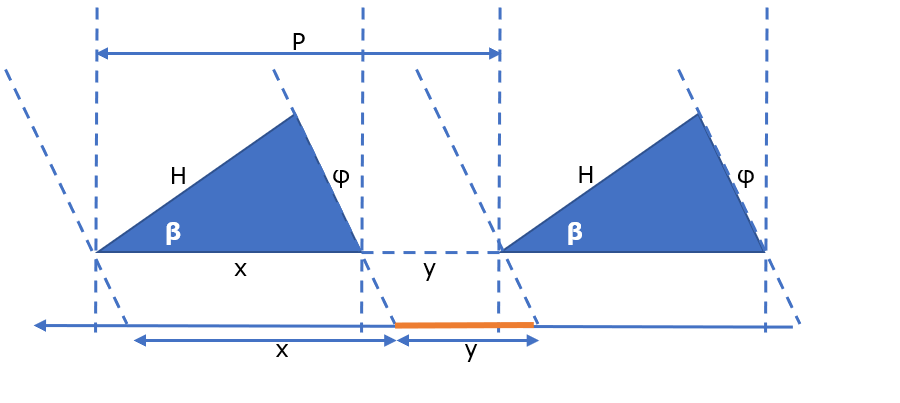
\includegraphics[width=9cm]{2d_infinite_sheds.png}
\caption{Two-dimensional infinitely long PV racks at tilt, $\beta$, each of length $H$, separated by distance $P$.  The vertical dashed lines are parallel to the z-axis, the arrow to the left is the y-axis, and the x-axis points into the page, forming a right-hand coordinate system.  The projection of the solar angle on the y-z plane is $\phi$. The shaded and illuminated regions beneath the racks are shown as $x$ and $y$, respectively.}
\end{figure}

We calculate backside irradiance by treating it as a surface tilted by the supplement of the front surface, and an azimuth that is rotated 180\degree\ around the zenith from the front surface.  The irradiance components for both surfaces can be calculated using any of the transposition models.  Fig. 2 and 3 show the irradiance components for the front and back surfaces of a PV rack calculated using several transposition models from pvlib-python \cite{Holmgren2018} with predicted clear sky irradiance at a latitude and longitude of (37.85\degree, -122.25\degree) on the morning of Jan. 1st, 2017.  The front surface is tilted 20\degree\ at an azimuth of 250\degree, so the back surface is tilted at 160\degree\ and the corresponding reference frame is at an azimuth of 70\degree.  The diffuse components are non-zero starting at sunrise at 7:25 PST, but the direct component doesn’t strike the front surface until 8:35 PST because it’s on the back side.

% Fig. 1
\begin{figure}
\centering
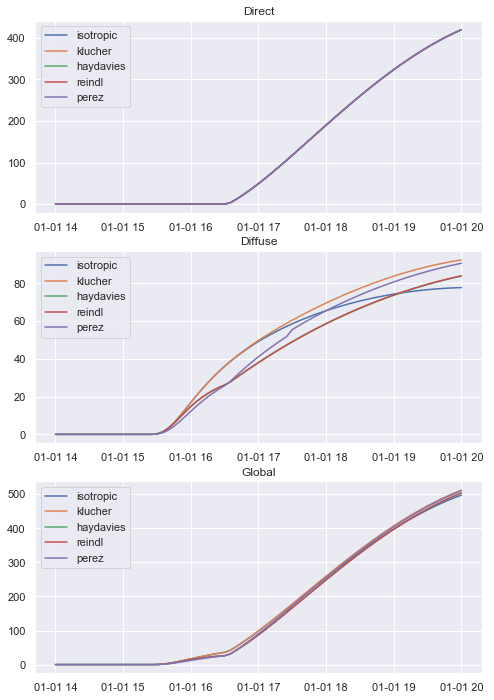
\includegraphics[width=9cm]{frontside_transposition.png}
\caption{Predicted plane of array components using different transposition models on the front surface of a rack tilted at 20\degree\ facing 250\degree\ and located at a latitude and longitude of (37.85\degree, -122.25\degree) on Jan. 1st, 2017.  The top panel shows direct irradiance, the middle shows combined diffuse irradiance from both sky and ground, and the bottom panel shows the total global irradiance on the plane of the array.}
\end{figure}

% Fig. 2
\begin{figure}
\centering
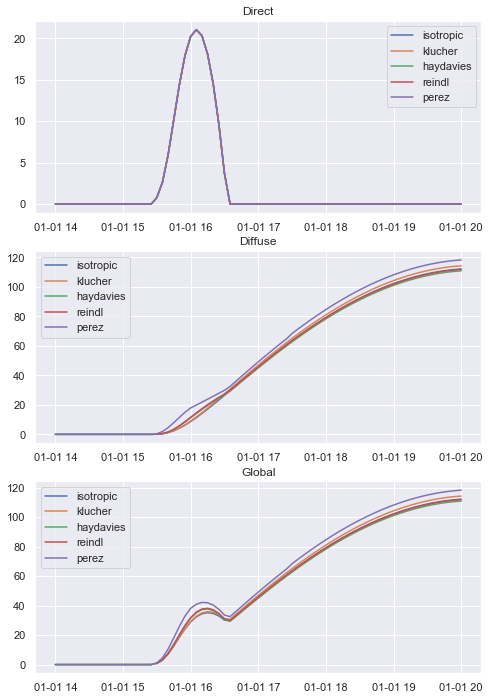
\includegraphics[width=9cm]{backside_transposition.png}
\caption{Predicted plane of array components using different transposition models on the back surface of a rack tilted at 160\degree\ facing 70\degree\ and located at a latitude and longitude of (37.85\degree, -122.25\degree) on Jan. 1st, 2017.  The top panel shows direct irradiance, the middle shows combined diffuse irradiance from both sky and ground, and the bottom panel shows the total global irradiance on the plane of the array.}
\end{figure}

Notice in the middle of Fig. 3 that the backside diffuse component is significantly overestimated because it doesn’t consider that the PV rack both shades the ground and blocks the sky, therefore reducing incident and reflected irradiance.

\subsection{ Ground Reflection with Shade and Obstructions}
The diffuse component of the irradiance on the back surface in Fig. 3 contains contributions from both the sky and ground reflection.  The ground reflection incident on the plane of array, $POA_{gnd}$, assuming no shading and no blocking, is given by the relation in (3) below with the global horizontal irradiance ($GHI$), the ground albedo ($\rho$), and the view factor from the ground to the PV surface, $F_{gnd,pv} = \frac{\left(1-\cos\beta\right)}{2}$ \cite{Marion2017}.

%Eq. 3
\begin{equation}
POA_{gnd} = \rho GHI \frac{\left(1-\cos \beta \right)}{2}
\end{equation}

The PV rack reduces the ground reflected irradiance both by shading the ground and blocking the sky.  We can account for shade on the ground by calculating the fraction of ground between each pair of rows, $F_{sky,gnd}$, with only incident direct irradiance. The fraction of unshaded ground is expressed in (4) as the ratio $\frac{y}{P}$, with unshaded ground $y$ and row spacing $P$ from Fig. 1.  The fraction of the shaded ground is then $1-F_{sky,gnd}$.

%Eq. 4
\begin{equation}
F_{sky,gnd} = 1 - \min(0,\ GCR \left| \cos \beta + \sin \beta \tan \phi \right|)
\end{equation}

The ground coverage ratio, $GCR$, is the ratio of the rack height to spacing, $\frac{H}{P}$, from Fig. 1.  The projected solar angle on the vertical plane perpendicular to the rows is expressed in (5) using solar zenith, $\theta$, solar azimuth, $\gamma$, and the orientation of the PV surface, $\gamma_{surface}$.

%Eq. 5
\begin{equation}
\tan \phi = \cos \left(\gamma - \gamma_{surface} \right) \tan \theta
\end{equation}

As shown in Fig. 4, the sky is blocked by the PV panels.  We can account for the blocked sky between each pair of rows by calculating the view factor of the sky from the ground, $F_{x \rightarrow sky}$ given by the angles $\psi_0(x)$ and $\psi_1\left(x\right)$ \cite{Marion2017}.

%Eq. 6
\begin{equation}
F_{x \rightarrow sky} = \frac{\cos \psi_1\left(x \right) + \cos \psi_1\left(x \right)}{2}
\end{equation}

% Fig. 4
\begin{figure}
\centering
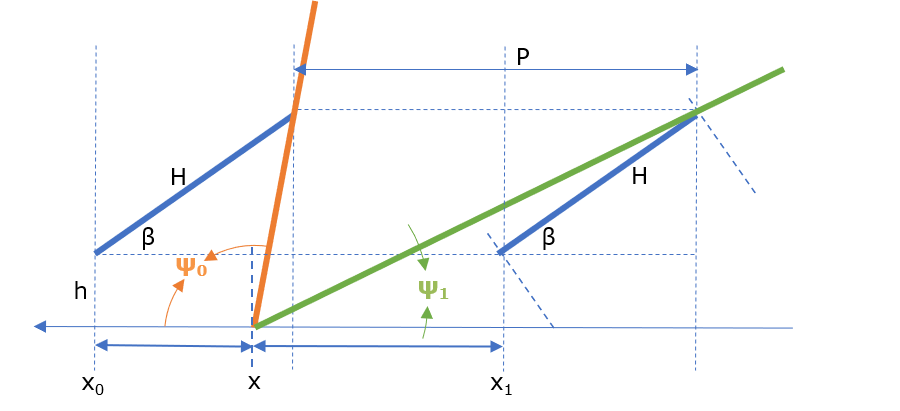
\includegraphics[width=9cm]{ground_sky_vf.png}
\caption{Two dimensional view of a pair of adjacent rows at $x_0$ and $x_1$ separated by spacing $P$, tilted by angle $\beta$, of height $H$, and at height $h$ above the ground.  The view of the sky at point $x$ on the ground is subtended by angles $\psi_0(x)$ and $\psi_1\left(x\right)$.}
\end{figure}

Note in Fig. 4 the angles are both measured from the ground in opposite directions.  If one of the angles is replaced with its supplement the view factor in (6) would be a difference of cosines instead of the sum, because $\cos \left(\pi - \alpha\right) = -\cos \alpha$.  However, defining the angles this makes their derivation easier, so for any $x$ the angles are given as follows:

%Eq. 7 & 8
\begin{align}
\tan \psi_0 &= \frac{\sin \beta^\prime}{\frac{F_x}{GCR^\prime} + \cos \beta^\prime}\\
\tan \psi_1 &= \frac{\sin \beta}{\frac{F_y}{GCR^\prime} + \cos \beta}
\end{align}

In (7), $\beta^\prime$ is the supplement of $\beta$ and $F_x$ is the fraction of the row spacing, $P$, from $x_0$ to $x$, in (7) and (8), $GCR^\prime=GCR+\frac{h}{P\sin\beta}$ to account for the height of the PV racks above the ground, $h$, and in (8), $F_y=1-F_x$ for convenience.

As the PV rack height is increased, the ground near $x_0$ and $x_1$ can see the sky between adjacent rows, although they are blocked by the bottom of the panel closest to that point.  We can derive the limiting angles from the top to the bottom of each row and vice versa, $\psi_{top}\left(x=0\right)$ and $\psi_{bottom}\left(y=0\right)$ in Fig. 6.  Examining the combined view factors for several heights and GCR values, shown in Fig 5, it seems that the net view factor for the space between rows can be approximated as the average of the zero height view factors at $x_0$ and $x_1$.

\begin{table}
\centerline { TABLE 1 } 
\vskip5pt
\centerline { \normalsize \textsc{Ground-Sky View Factor vs. Height}}
\vskip2pt
\centerline{
\vbox{\offinterlineskip
\hrule
%\vskip2pt\hrule\vskip2pt
% Leading & means preamble template repeats infinitely. p.241 TeX Book.
\halign{&\vrule#&
\strut\quad#\hfil\quad\cr
%Use either first and third lines following this description, OR the
%second line.  The first choice is used when all vertical rules go to the
%top of the first horizontal line of the table.  The second choice below
%(with the \strut) is used when there are column headings that span
%more than one column.  The \strut in that column line will not have the
%vertical tic marks in the horizontal rule.  Note that a vrule is also
%considered a column, so when using \multispanx, x is the number of
%all columns including the ``vrule.'' 
height2pt&\omit&&\omit&&\omit&&\omit&&\omit&\cr
%&\strut &&\multispan5\hfil {\bf Font Specifics}\hfil&&\multispan9\hfil {\bf Paragraph Description}\hfil &\cr
%&\omit &&\multispan5\hfil {\bf Font Specifics}\hfil&&\multispan9\hfil {\bf Paragraph Description}\hfil &\cr
%&{\bf Section}&&\multispan5\hfil (Times Roman unless
%specified)\hfil&&\multispan5\hfil spacing (in points)\hfil &&
%alignment&&indent&\cr
&\omit&&style&&size&&special&&line&\cr
height2pt&\omit&&\omit&&\omit&&\omit&&\omit&\cr
\noalign{\hrule}
height2pt&\omit&&\omit&&\omit&&\omit&&\omit&\cr
%\noalign{\vskip2pt\hrule\vskip2pt}
%\omit&\omit&\omit&\omit\cr
&Title&&plain&&18&&none&&single&\cr
&Author List&&plain&&12&&none&&single&\cr
&Affiliations&&plain&&12&&none&&single&\cr
&Abstract&&bold&&9&&none&&exactly 10&\cr
&Headings&&plain&&10&&small caps&&exactly 12&&\cr
&Subheadings&&italic&&10&&none&&exactly 12&\cr
&Body Paragraphs&&plain&&10&&none&&exactly 12&\cr
&Figure Captions&&plain&&9&&none &&10&\cr
&References&&plain&&9&&none&&10&\cr
height2pt&\omit&&\omit&&\omit&&\omit&&\omit&\cr}
\hrule}}
\label{table1}
\end{table}

%\begin{figure}
%%\includegraphics {figure_temp.epsi}
%\epsfxsize=3.25in\epsfbox{figure1.eps}
%\caption{ Estimated relationship between the time an author spends reading these instructions and the quality of the author's digest article.}
%\end{figure}

%\LaTeX accepts encapsulated post script files as figures.  Standard post script figures will not expand and contract to fill the designate area on the page. Encapsulated post script files will.  Thus, encapsulated post script files must obviously be only one page long.  It is often easy to convert a post script file to encapsulated post script.  In Linux this can be done with the command, ``ps2epsi.''
%More flexibility is obtained in inserting figures if you can place
%them exactly where you would like them to be on a page. This can be
%accomplished by inserting the figure, selecting the figure, and then
%choosing ``Format Picture\dots ''. Various settings allow you to place the figure at an absolute position on a page; specify if the text is supposed to flow around the figure or if the figure should move with the text, etc. If you elect to let the text flow around the figure, then remember that you will have to insert a separate text box for the caption, otherwise the figure caption is likely to become separated from the figure.
%When importing a graph from Excel into Word, it is often helpful to
%special-paste it in as a ``Picture (Enhanced Meta-file).'' This saves
%file memory for Word documents. Be aware that the usual Copy
%$\rightarrow $  Paste procedure will copy the entire Excel spreadsheet into your Word file. The Copy $\rightarrow$ Paste Special $\rightarrow$ Picture (Enhanced Metafile) command copies only the graph as a static picture. This is not a concern with PDF file submissions.

We can approximate the ground reflection from the shaded ground by applying the albedo to the diffuse horizontal irradiance, $DHI$.  Then the reflected irradiance from the ground with shade, $POA_{gnd,shade}$, incident on the back surface is the sum from shaded and unshaded ground, where $DHI/GHI$ is the diffuse ratio, $df$.  This doesn’t consider the obstruction by the adjacent rows of the view from the current row to the ground and sky.

It is also important to consider the effect of the width of the sun on the fraction of shaded ground. The radius of the solar disc is about 4.65-milliradians or 0.266\degree\ which would decrease the size of the shadow by about 10-cm per meter as the height of the PV rack was increased.

\section{Citing Previous Work}

% Fig. 5
\begin{figure}
\centering
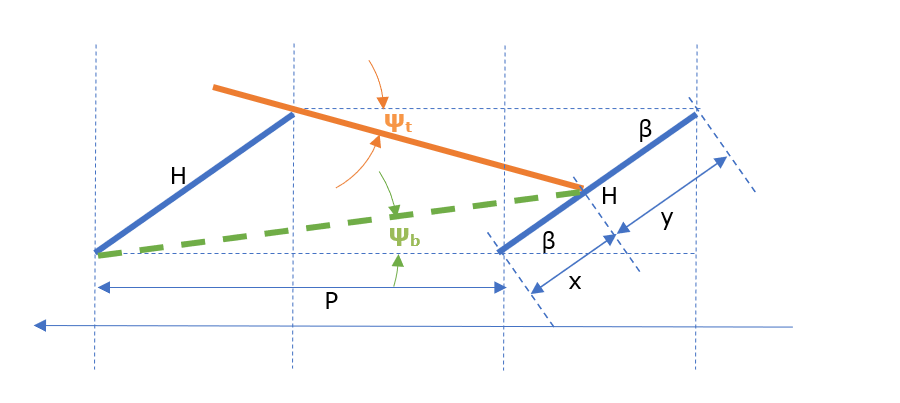
\includegraphics[width=9cm]{next-row-view-factor-angles.png}
\caption{Example of readable plot using different colors and line styles for clarity.}
\end{figure}

When referencing a journal article \cite{Mikofski_8547323}, a conference
digest article \cite{Mikofski_8547323} or a book \cite{Mikofski_8547323}, place the reference numbers within square
brackets. To simultaneously cite these references \cite{Mikofski_8547323} - \cite{Mikofski_8547323} use the format just demonstrated. The reference list is the last section and references are listed in the order cited. Use 9 point Times. The paragraph description is set for a line spacing of exactly 10 points with 0 point spacing before and after. A 0.25 inch hanging indention should be specified. 

Generally speaking, references should be very detailed. For journal articles, list all authors by initials and last name, the title of the paper in quotations (capitalizing only the first letter of the first word, unless it would be capitalized in a sentence, e.g., a proper noun), the journal name in italics, the volume number, the issue number, the page numbers, and the date. Use the examples provided \cite{Mikofski_8547323} - \cite{Mikofski_8547323} as a guide. 
%Further information on LaTeX and TeX can be found in \cite{IEEEhowto:kopka} - \cite{knuth}. 

% The following statement makes the two columns on the last page more
% or less of equal length.  Placement of this command is by trial and error.
\vfil\eject

\section{Copyright and Reprint Information}
The IEEE copyright form will be electronically submitted for this conference.  On the conference web site, follow the link in the manuscript submission area. 

Reprints may be ordered by checking the appropriate box on the conference registration form.  The reprints will be mailed to you at the address listed on the registration form approximately 3 months after the conference.


\section{Conclusion}
Following these instructions will improve the quality of your paper and the PVSC Proceedings. If you have comments, please contact \url{Publications@ieee-pvsc.org}. Please direct questions regarding the electronic submission process to \url{help@SPLTrak.com}. 

% conference papers do not normally have an appendix

% use section* for acknowledgment



% conference papers do not normally have an appendix


% use section* for acknowledgement



% trigger a \newpage just before the given reference
% number - used to balance the columns on the last page
% adjust value as needed - may need to be readjusted if
% the document is modified later
%\IEEEtriggeratref{8}
% The "triggered" command can be changed if desired:
%\IEEEtriggercmd{\enlargethispage{-5in}}

% references section

% can use a bibliography generated by BibTeX as a .bbl file
% BibTeX documentation can be easily obtained at:
% http://www.ctan.org/tex-archive/biblio/bibtex/contrib/doc/
% The IEEEtran BibTeX style support page is at:
% http://www.michaelshell.org/tex/ieeetran/bibtex/
\bibliographystyle{IEEEtran}
% argument is your BibTeX string definitions and bibliography database(s)
\bibliography{IEEEabrv,C:/Users/mikm/Projects/pvsc46/bibliography}
%
% <OR> manually copy in the resultant .bbl file
% set second argument of \begin to the number of references
% (used to reserve space for the reference number labels box)

%\begin{thebibliography}{1}
%\small

%\bibitem {Yamaguchi}
%M. Yamaguchi, A. Khan, S.J. Taylor, M. Imaizumi, T. Hisamatsu, and S. Matsuda, ``A detailed model to improve the radiation-resistance of Si space solar cells,\emph{Fundamentals of Solar Cells} vol. 46, pp. 2133-2138, 1999.

%\bibitem {Hovel}
%H. J. Hovel and J. M. Woodall, ``The effect of depletion region recombination currents on the efficiencies of Si and GaAs solar cells'', \emph {in 10th IEEE Photovoltaic Specialist Conference}, p. 25, 1973.

%\bibitem {Fahrenbruch}
%A. L. Fahrenbruch and R. H. Bube, \emph{Fundamentals of Solar Cells}, New York: Academic Press, 1983.

%\bibitem{IEEEhowto:kopka}
%H.~Kopka and P.~W. Daly, \emph{A Guide to \LaTeX}, 3rd~ed.\hskip 1em plus
%  0.5em minus 0.4em\relax Harlow, England: Addison-Wesley, 1999.

%\end{thebibliography}
%\smallskip
%Note: For the Summary paper submission only, references to the authors own work must be redacted to preserve the new double-blind reviewing requirements.





% that's all folks
\end{document}


